\section{Unbiased $f_i$ Estimation}
\label{sec:unbiased-estimate}

Based on our observations in the previous section we will alter Kmerlight 
to produce unbiased estimates of $f_i$ (under the assumption that there are no undetedected
collisions).

To achieve an unbiased estimate of $f_i$ we will use the level that maximizes the
expected number number of collision-free counters, instead of the level that maximzes the number
of collision-free counters. We will base our estimates of $f_i$ on the level $w^+$, 
instead of $w_i^*$. Our modified Kmerlight thus loses the ability to choose the maximal 
$t^{(w)}$, and the estimates will be now based on values of $t^{(w^+)}$ which
are expected to vary evenly around their mean $E(t^{(w^+)})$, reaching both higher
and lower values than $E(t^{(w^+)})$.

Note that the value of $\hat f_i$ will be calculated from the same level for every abundance $i$.
Level $w^+$ will be calculated using only the estimated number of all distinct $k$-mers ($F_0$)
and the number of counters at each level ($r$).

Modified Kmerlight first processes all the $k$-mers in the same
way as the original Kmerlight. Then $F_0$ is estimated from all Kmerlight's instances\footnote{
The value of $F_0$ is estimated in the original way as presented in (\ref{eq:hatF0}).
Note that the estimate depends on the value of $t_0^{(w)}$, $E(t_0^{(w)}) = r \cdot p_e$. 
Number of empty counters reach high values ($t_0^{(w^*)} \approx r/2$) thus $t_0$ has low
relative variance and so the effects that biased $\hat f_i$ do not occur here or they cause 
a smaller scale differences. We do no challenge the unbiasdness of the estimator $\hat F_0$
in our work.
}
and the value $w^+$ is calculated to maximize the expected number of
collision-free counters as it was described in section \ref{sec:analytical-w}.
Finally, values of $f_i$ are estimated from the observed counts of 
collision-free counters at level $w^+$ by (\ref{eq:hatfi}).

In figures \ref{img:mean-new-algorithm} and \ref{img:std-new-algorithm}, we present a comparison
of the original Kmerlight and the modified Kmerlight. We ran both versions of Kmerlight
on the same data as described in \ref{sec:error-characteristics} in 300 trials. 
Our new algorithm removes bias and maintains the same accuracy (variance) of the estimates.

\begin{figure}[h!]
\centerline{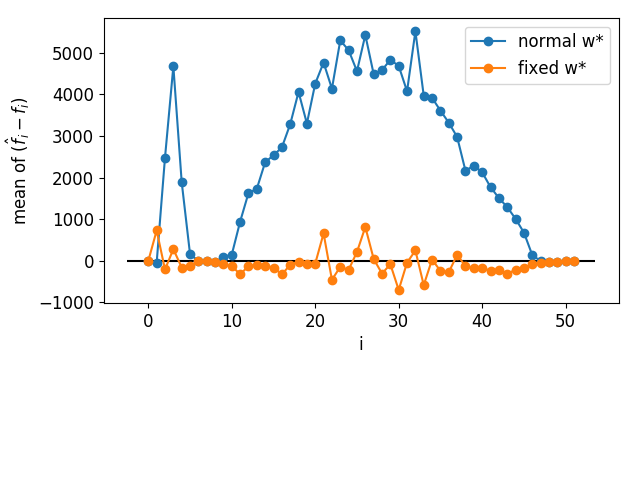
\includegraphics[width=0.8\textwidth, trim={0cm, 3.5cm, 0cm, 0cm}, clip]{images/means_comparison.png}}
\caption[Mean error of the original Kmerlight and the modified Kmerlight]{Mean errors of estimates
($\hat f_i - f_i$) produced by original (blue) and modified (orange) Kmerlight in 300 trials. 
While the original Kmerlight overestimates $f_i$ significantly in an average run,
modified Kmerlight achieves $E(\hat f_i) \approx f_i$.}
\label{img:mean-new-algorithm}
\end{figure}

\begin{figure}[h!]
\centerline{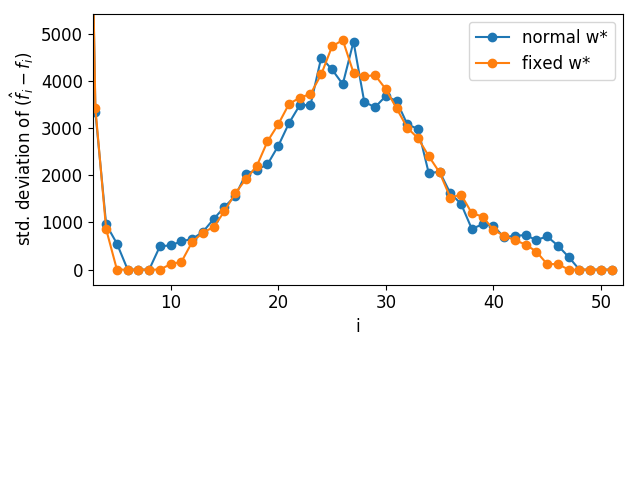
\includegraphics[width=0.8\textwidth, trim={0cm, 4.3cm, 0cm, 0cm}, clip]{images/std_deviations_comparison.png}}
\caption[Variance of the original Kmerlight and the modified Kmerlight]{Standard deviation
of estimates ($\hat f_i - f_i$) produced by original (blue) and modified (orange) Kmerlight 
in 300 trials. Our modification of Kmerlight does not change the variance of estimates.}
\label{img:std-new-algorithm}
\end{figure}

\paragraph{Decreased memory consumption}
Note that we used only one of $64$ Kmerlight's levels to compute estimates for all $f_i$.
We cannot decrease the overall memory consumption by a factor of 64, however. 
To compute $\hat F_0$, more levels are needed, but still, we can compute the estimate
of $F_0$ separately from the estimates of $f_i$.

If we roughly guess $F_0$ from the size of sequencing data, we might be able
to estimate $F_0$ with a lower number of levels. It might be also sufficient
to estimate $F_0$ with smaller arrays of conters at each level (smaller parameter $r$).
Also a completely different method might be used for $F_0$ computation.

We did not inquire deeper into the topic of decreasing the memory consumption,
but we believe that at least a tenfold improvement might be achieved in this direction.